\documentclass[twoside]{book}

% Packages required by doxygen
\usepackage{fixltx2e}
\usepackage{calc}
\usepackage{doxygen}
\usepackage[export]{adjustbox} % also loads graphicx
\usepackage{graphicx}
\usepackage[utf8]{inputenc}
\usepackage{makeidx}
\usepackage{multicol}
\usepackage{multirow}
\PassOptionsToPackage{warn}{textcomp}
\usepackage{textcomp}
\usepackage[nointegrals]{wasysym}
\usepackage[table]{xcolor}

% Font selection
\usepackage[T1]{fontenc}
\usepackage[scaled=.90]{helvet}
\usepackage{courier}
\usepackage{amssymb}
\usepackage{sectsty}
\renewcommand{\familydefault}{\sfdefault}
\allsectionsfont{%
  \fontseries{bc}\selectfont%
  \color{darkgray}%
}
\renewcommand{\DoxyLabelFont}{%
  \fontseries{bc}\selectfont%
  \color{darkgray}%
}
\newcommand{\+}{\discretionary{\mbox{\scriptsize$\hookleftarrow$}}{}{}}

% Page & text layout
\usepackage{geometry}
\geometry{%
  a4paper,%
  top=2.5cm,%
  bottom=2.5cm,%
  left=2.5cm,%
  right=2.5cm%
}
\tolerance=750
\hfuzz=15pt
\hbadness=750
\setlength{\emergencystretch}{15pt}
\setlength{\parindent}{0cm}
\setlength{\parskip}{3ex plus 2ex minus 2ex}
\makeatletter
\renewcommand{\paragraph}{%
  \@startsection{paragraph}{4}{0ex}{-1.0ex}{1.0ex}{%
    \normalfont\normalsize\bfseries\SS@parafont%
  }%
}
\renewcommand{\subparagraph}{%
  \@startsection{subparagraph}{5}{0ex}{-1.0ex}{1.0ex}{%
    \normalfont\normalsize\bfseries\SS@subparafont%
  }%
}
\makeatother

% Headers & footers
\usepackage{fancyhdr}
\pagestyle{fancyplain}
\fancyhead[LE]{\fancyplain{}{\bfseries\thepage}}
\fancyhead[CE]{\fancyplain{}{}}
\fancyhead[RE]{\fancyplain{}{\bfseries\leftmark}}
\fancyhead[LO]{\fancyplain{}{\bfseries\rightmark}}
\fancyhead[CO]{\fancyplain{}{}}
\fancyhead[RO]{\fancyplain{}{\bfseries\thepage}}
\fancyfoot[LE]{\fancyplain{}{}}
\fancyfoot[CE]{\fancyplain{}{}}
\fancyfoot[RE]{\fancyplain{}{\bfseries\scriptsize Generated by Doxygen }}
\fancyfoot[LO]{\fancyplain{}{\bfseries\scriptsize Generated by Doxygen }}
\fancyfoot[CO]{\fancyplain{}{}}
\fancyfoot[RO]{\fancyplain{}{}}
\renewcommand{\footrulewidth}{0.4pt}
\renewcommand{\chaptermark}[1]{%
  \markboth{#1}{}%
}
\renewcommand{\sectionmark}[1]{%
  \markright{\thesection\ #1}%
}

% Indices & bibliography
\usepackage{natbib}
\usepackage[titles]{tocloft}
\setcounter{tocdepth}{3}
\setcounter{secnumdepth}{5}
\makeindex

% Hyperlinks (required, but should be loaded last)
\usepackage{ifpdf}
\ifpdf
  \usepackage[pdftex,pagebackref=true]{hyperref}
\else
  \usepackage[ps2pdf,pagebackref=true]{hyperref}
\fi
\hypersetup{%
  colorlinks=true,%
  linkcolor=blue,%
  citecolor=blue,%
  unicode%
}

% Custom commands
\newcommand{\clearemptydoublepage}{%
  \newpage{\pagestyle{empty}\cleardoublepage}%
}

\usepackage{caption}
\captionsetup{labelsep=space,justification=centering,font={bf},singlelinecheck=off,skip=4pt,position=top}

%===== C O N T E N T S =====

\begin{document}

% Titlepage & ToC
\hypersetup{pageanchor=false,
             bookmarksnumbered=true,
             pdfencoding=unicode
            }
\pagenumbering{alph}
\begin{titlepage}
\vspace*{7cm}
\begin{center}%
{\Large P\+S\+E\+Mol\+Dyn\+\_\+\+GroupG \\[1ex]\large 2 }\\
\vspace*{1cm}
{\large Generated by Doxygen 1.8.14}\\
\end{center}
\end{titlepage}
\clearemptydoublepage
\pagenumbering{roman}
\tableofcontents
\clearemptydoublepage
\pagenumbering{arabic}
\hypersetup{pageanchor=true}

%--- Begin generated contents ---
\chapter{Hierarchical Index}
\section{Class Hierarchy}
This inheritance list is sorted roughly, but not completely, alphabetically\+:\begin{DoxyCompactList}
\item \contentsline{section}{File\+Reader}{\pageref{class_file_reader}}{}
\item \contentsline{section}{Input}{\pageref{class_input}}{}
\item \contentsline{section}{Iterator$<$ Item $>$}{\pageref{class_iterator}}{}
\item \contentsline{section}{Iterator$<$ Particle $>$}{\pageref{class_iterator}}{}
\begin{DoxyCompactList}
\item \contentsline{section}{Particle\+Iterator}{\pageref{class_particle_iterator}}{}
\end{DoxyCompactList}
\item \contentsline{section}{Particle}{\pageref{class_particle}}{}
\item \contentsline{section}{particle\+Generator}{\pageref{classparticle_generator}}{}
\end{DoxyCompactList}

\chapter{Class Index}
\section{Class List}
Here are the classes, structs, unions and interfaces with brief descriptions\+:\begin{DoxyCompactList}
\item\contentsline{section}{\mbox{\hyperlink{class_file_reader}{File\+Reader}} }{\pageref{class_file_reader}}{}
\item\contentsline{section}{\mbox{\hyperlink{class_input}{Input}} }{\pageref{class_input}}{}
\item\contentsline{section}{\mbox{\hyperlink{class_iterator}{Iterator$<$ Item $>$}} }{\pageref{class_iterator}}{}
\item\contentsline{section}{\mbox{\hyperlink{class_particle}{Particle}} }{\pageref{class_particle}}{}
\item\contentsline{section}{\mbox{\hyperlink{classparticle_generator}{particle\+Generator}} }{\pageref{classparticle_generator}}{}
\item\contentsline{section}{\mbox{\hyperlink{class_particle_iterator}{Particle\+Iterator}} }{\pageref{class_particle_iterator}}{}
\end{DoxyCompactList}

\chapter{Class Documentation}
\hypertarget{class_file_reader}{}\section{File\+Reader Class Reference}
\label{class_file_reader}\index{File\+Reader@{File\+Reader}}
\subsection*{Public Member Functions}
\begin{DoxyCompactItemize}
\item 
\mbox{\Hypertarget{class_file_reader_a98e0f676c498629dd005101f399f2a3c}\label{class_file_reader_a98e0f676c498629dd005101f399f2a3c}} 
void {\bfseries read\+File} (std\+::list$<$ \mbox{\hyperlink{class_particle}{Particle}} $>$ \&particles, char $\ast$filename)
\item 
\mbox{\Hypertarget{class_file_reader_a56efd05cfd8e7b6489ac406372b55d67}\label{class_file_reader_a56efd05cfd8e7b6489ac406372b55d67}} 
void {\bfseries read\+File2} (std\+::list$<$ \mbox{\hyperlink{classparticle_generator}{particle\+Generator}} $>$ \&a, std\+::list$<$ utils\+::\+Vector$<$ double, 3 $>$$>$ \&b, double \&end\+\_\+time, double \&delta\+\_\+t, char $\ast$filename)
\end{DoxyCompactItemize}


The documentation for this class was generated from the following files\+:\begin{DoxyCompactItemize}
\item 
src/File\+Reader.\+h\item 
src/File\+Reader.\+cpp\end{DoxyCompactItemize}

\hypertarget{class_input}{}\section{Input Class Reference}
\label{class_input}\index{Input@{Input}}
\subsection*{Public Member Functions}
\begin{DoxyCompactItemize}
\item 
\mbox{\Hypertarget{class_input_aceecd12aad47433477cfc32743c41743}\label{class_input_aceecd12aad47433477cfc32743c41743}} 
std\+::list$<$ \mbox{\hyperlink{class_particle}{Particle}} $>$ {\bfseries Interpret\+Input} (int c, char $\ast$param\mbox{[}$\,$\mbox{]})
\end{DoxyCompactItemize}
\subsection*{Public Attributes}
\begin{DoxyCompactItemize}
\item 
\mbox{\Hypertarget{class_input_a3d93c2a1146f4e8f544208d6d68073e5}\label{class_input_a3d93c2a1146f4e8f544208d6d68073e5}} 
double {\bfseries end\+\_\+timei}
\item 
\mbox{\Hypertarget{class_input_a2e63e0524d1a0648e6d1b805fff41c5d}\label{class_input_a2e63e0524d1a0648e6d1b805fff41c5d}} 
double {\bfseries delta\+\_\+ti}
\end{DoxyCompactItemize}


The documentation for this class was generated from the following files\+:\begin{DoxyCompactItemize}
\item 
src/Input.\+h\item 
src/Input.\+cpp\end{DoxyCompactItemize}

\hypertarget{class_iterator}{}\section{Iterator$<$ Item $>$ Class Template Reference}
\label{class_iterator}\index{Iterator$<$ Item $>$@{Iterator$<$ Item $>$}}
\subsection*{Public Member Functions}
\begin{DoxyCompactItemize}
\item 
\mbox{\Hypertarget{class_iterator_ab50d3d7ae6eea85b3a0d5d772634e26b}\label{class_iterator_ab50d3d7ae6eea85b3a0d5d772634e26b}} 
virtual void {\bfseries First} ()=0
\item 
\mbox{\Hypertarget{class_iterator_abd77d09a88909400b65ab95a55a636cf}\label{class_iterator_abd77d09a88909400b65ab95a55a636cf}} 
virtual void {\bfseries Next} ()=0
\item 
\mbox{\Hypertarget{class_iterator_ac4c54c80c84ac3c3dbd75942fcb81671}\label{class_iterator_ac4c54c80c84ac3c3dbd75942fcb81671}} 
virtual bool {\bfseries Is\+Done} () const =0
\item 
\mbox{\Hypertarget{class_iterator_a1ae60208b26a4ae33f57181806816a33}\label{class_iterator_a1ae60208b26a4ae33f57181806816a33}} 
virtual Item {\bfseries Current\+Item} () const =0
\end{DoxyCompactItemize}


The documentation for this class was generated from the following file\+:\begin{DoxyCompactItemize}
\item 
src/Particle.\+cpp\end{DoxyCompactItemize}

\hypertarget{class_particle}{}\section{Particle Class Reference}
\label{class_particle}\index{Particle@{Particle}}
\subsection*{Public Member Functions}
\begin{DoxyCompactItemize}
\item 
\mbox{\Hypertarget{class_particle_a866812d3dfb9c539e5e24593e596a8c9}\label{class_particle_a866812d3dfb9c539e5e24593e596a8c9}} 
{\bfseries Particle} (int type=0)
\item 
\mbox{\Hypertarget{class_particle_a24b04cb7c6f7ea4242d25c410f44ae56}\label{class_particle_a24b04cb7c6f7ea4242d25c410f44ae56}} 
{\bfseries Particle} (const \mbox{\hyperlink{class_particle}{Particle}} \&other)
\item 
\mbox{\hyperlink{class_particle_a5a5b07aa732c302b45e90c12723f2b27}{Particle}} (utils\+::\+Vector$<$ double, 3 $>$ x\+\_\+arg, utils\+::\+Vector$<$ double, 3 $>$ v\+\_\+arg, double m\+\_\+arg, int type=0)
\item 
virtual \mbox{\hyperlink{class_particle_ad030d0fe7b88cf81744b127c99244ff4}{$\sim$\+Particle}} ()
\item 
\mbox{\Hypertarget{class_particle_ab7ade5dc156dfa0234aa0323564e46ed}\label{class_particle_ab7ade5dc156dfa0234aa0323564e46ed}} 
utils\+::\+Vector$<$ double, 3 $>$ \& {\bfseries getX} ()
\item 
\mbox{\Hypertarget{class_particle_acd84c445e2bd5f5280a00e76cfe73fe0}\label{class_particle_acd84c445e2bd5f5280a00e76cfe73fe0}} 
utils\+::\+Vector$<$ double, 3 $>$ \& {\bfseries getF} ()
\item 
\mbox{\Hypertarget{class_particle_a1204435fc08c697b0fea230616d1bbdf}\label{class_particle_a1204435fc08c697b0fea230616d1bbdf}} 
utils\+::\+Vector$<$ double, 3 $>$ \& {\bfseries get\+OldF} ()
\item 
\mbox{\Hypertarget{class_particle_aaf3ecbc6e1e31b259fe239461ba13dbd}\label{class_particle_aaf3ecbc6e1e31b259fe239461ba13dbd}} 
utils\+::\+Vector$<$ double, 3 $>$ \& {\bfseries getV} ()
\item 
\mbox{\Hypertarget{class_particle_aa1ca800f9be9dd4bd6c604f608095b24}\label{class_particle_aa1ca800f9be9dd4bd6c604f608095b24}} 
double {\bfseries getM} ()
\item 
\mbox{\Hypertarget{class_particle_a0581d7b629eb17ac5bef8e934852ca8b}\label{class_particle_a0581d7b629eb17ac5bef8e934852ca8b}} 
int {\bfseries get\+Type} ()
\item 
\mbox{\Hypertarget{class_particle_a5034babb77618a56e00927d8891afabe}\label{class_particle_a5034babb77618a56e00927d8891afabe}} 
bool {\bfseries operator==} (\mbox{\hyperlink{class_particle}{Particle}} \&other)
\item 
\mbox{\Hypertarget{class_particle_a07d071a0f91f8ce7413201a6db3afe7b}\label{class_particle_a07d071a0f91f8ce7413201a6db3afe7b}} 
std\+::string {\bfseries to\+String} ()
\end{DoxyCompactItemize}


\subsection{Constructor \& Destructor Documentation}
\mbox{\Hypertarget{class_particle_a5a5b07aa732c302b45e90c12723f2b27}\label{class_particle_a5a5b07aa732c302b45e90c12723f2b27}} 
\index{Particle@{Particle}!Particle@{Particle}}
\index{Particle@{Particle}!Particle@{Particle}}
\subsubsection{\texorpdfstring{Particle()}{Particle()}}
{\footnotesize\ttfamily Particle\+::\+Particle (\begin{DoxyParamCaption}\item[{utils\+::\+Vector$<$ double, 3 $>$}]{x\+\_\+arg,  }\item[{utils\+::\+Vector$<$ double, 3 $>$}]{v\+\_\+arg,  }\item[{double}]{m\+\_\+arg,  }\item[{int}]{type = {\ttfamily 0} }\end{DoxyParamCaption})}

std\+::cout $<$$<$ \char`\"{}\+Particle generated!\char`\"{} $<$$<$ std\+::endl; \mbox{\Hypertarget{class_particle_ad030d0fe7b88cf81744b127c99244ff4}\label{class_particle_ad030d0fe7b88cf81744b127c99244ff4}} 
\index{Particle@{Particle}!````~Particle@{$\sim$\+Particle}}
\index{````~Particle@{$\sim$\+Particle}!Particle@{Particle}}
\subsubsection{\texorpdfstring{$\sim$\+Particle()}{~Particle()}}
{\footnotesize\ttfamily Particle\+::$\sim$\+Particle (\begin{DoxyParamCaption}{ }\end{DoxyParamCaption})\hspace{0.3cm}{\ttfamily [virtual]}}

0std\+::cout $<$$<$ \char`\"{}\+Particle destructed!\char`\"{} $<$$<$ std\+::endl; 

The documentation for this class was generated from the following files\+:\begin{DoxyCompactItemize}
\item 
src/Particle.\+h\item 
src/Particle.\+cpp\end{DoxyCompactItemize}

\hypertarget{classparticle_generator}{}\section{particle\+Generator Class Reference}
\label{classparticle_generator}\index{particle\+Generator@{particle\+Generator}}
\subsection*{Public Member Functions}
\begin{DoxyCompactItemize}
\item 
\mbox{\Hypertarget{classparticle_generator_af17795ad0318c8b3a9252f3cd4d08b8c}\label{classparticle_generator_af17795ad0318c8b3a9252f3cd4d08b8c}} 
{\bfseries particle\+Generator} (utils\+::\+Vector$<$ double, 3 $>$ c, utils\+::\+Vector$<$ double, 3 $>$ d, int h, int m, utils\+::\+Vector$<$ double, 3 $>$ v, utils\+::\+Vector$<$ double, 3 $>$ bm)
\item 
int \& \mbox{\hyperlink{classparticle_generator_a15769993d769d9ca466eb5d68f3acad2}{create\+Grid}} (std\+::list$<$ \mbox{\hyperlink{class_particle}{Particle}} $>$ \&particles, double factor)
\item 
\mbox{\Hypertarget{classparticle_generator_a49119d0737c3626c80e6c7568a50dba0}\label{classparticle_generator_a49119d0737c3626c80e6c7568a50dba0}} 
int \& {\bfseries multi\+Grids} (std\+::list$<$ \mbox{\hyperlink{class_particle}{Particle}} $>$ \&a, double factor)
\end{DoxyCompactItemize}
\subsection*{Static Public Member Functions}
\begin{DoxyCompactItemize}
\item 
\mbox{\Hypertarget{classparticle_generator_aebfd96dacf007343af19281ec5a65593}\label{classparticle_generator_aebfd96dacf007343af19281ec5a65593}} 
static utils\+::\+Vector$<$ double, 3 $>$ {\bfseries calculate\+Mean\+Val} (utils\+::\+Vector$<$ double, 3 $>$ x, double m, double factor)
\end{DoxyCompactItemize}
\subsection*{Public Attributes}
\begin{DoxyCompactItemize}
\item 
\mbox{\Hypertarget{classparticle_generator_ab80e773221f217a33d4b1be568e83c38}\label{classparticle_generator_ab80e773221f217a33d4b1be568e83c38}} 
utils\+::\+Vector$<$ double, 3 $>$ {\bfseries velocity\+BM}
\item 
\mbox{\Hypertarget{classparticle_generator_a5871f5ebe841c2b1c5fb1f2204301ae6}\label{classparticle_generator_a5871f5ebe841c2b1c5fb1f2204301ae6}} 
utils\+::\+Vector$<$ double, 3 $>$ {\bfseries coordinates}
\item 
\mbox{\Hypertarget{classparticle_generator_a9732889f7714a7ffc9c534a9f4697743}\label{classparticle_generator_a9732889f7714a7ffc9c534a9f4697743}} 
utils\+::\+Vector$<$ double, 3 $>$ {\bfseries dimensions}
\item 
\mbox{\Hypertarget{classparticle_generator_a2495fe784adc4df5efe64792aba897c1}\label{classparticle_generator_a2495fe784adc4df5efe64792aba897c1}} 
int {\bfseries mesh\+\_\+width}
\item 
\mbox{\Hypertarget{classparticle_generator_ace647dfea1735c36a0201aa389985b16}\label{classparticle_generator_ace647dfea1735c36a0201aa389985b16}} 
int {\bfseries mass}
\item 
\mbox{\Hypertarget{classparticle_generator_ac186888d269707c311d5721b4ad9a0c5}\label{classparticle_generator_ac186888d269707c311d5721b4ad9a0c5}} 
utils\+::\+Vector$<$ double, 3 $>$ {\bfseries velocity}
\end{DoxyCompactItemize}


\subsection{Member Function Documentation}
\mbox{\Hypertarget{classparticle_generator_a15769993d769d9ca466eb5d68f3acad2}\label{classparticle_generator_a15769993d769d9ca466eb5d68f3acad2}} 
\index{particle\+Generator@{particle\+Generator}!create\+Grid@{create\+Grid}}
\index{create\+Grid@{create\+Grid}!particle\+Generator@{particle\+Generator}}
\subsubsection{\texorpdfstring{create\+Grid()}{createGrid()}}
{\footnotesize\ttfamily int \& particle\+Generator\+::create\+Grid (\begin{DoxyParamCaption}\item[{std\+::list$<$ \mbox{\hyperlink{class_particle}{Particle}} $>$ \&}]{particles,  }\item[{double}]{factor }\end{DoxyParamCaption})}

std\+::cout$<$$<$i$<$$<$std\+::endl; 

The documentation for this class was generated from the following files\+:\begin{DoxyCompactItemize}
\item 
src/particle\+Generator.\+h\item 
src/particle\+Generator.\+cpp\end{DoxyCompactItemize}

\hypertarget{class_particle_iterator}{}\section{Particle\+Iterator Class Reference}
\label{class_particle_iterator}\index{Particle\+Iterator@{Particle\+Iterator}}
Inheritance diagram for Particle\+Iterator\+:\begin{figure}[H]
\begin{center}
\leavevmode
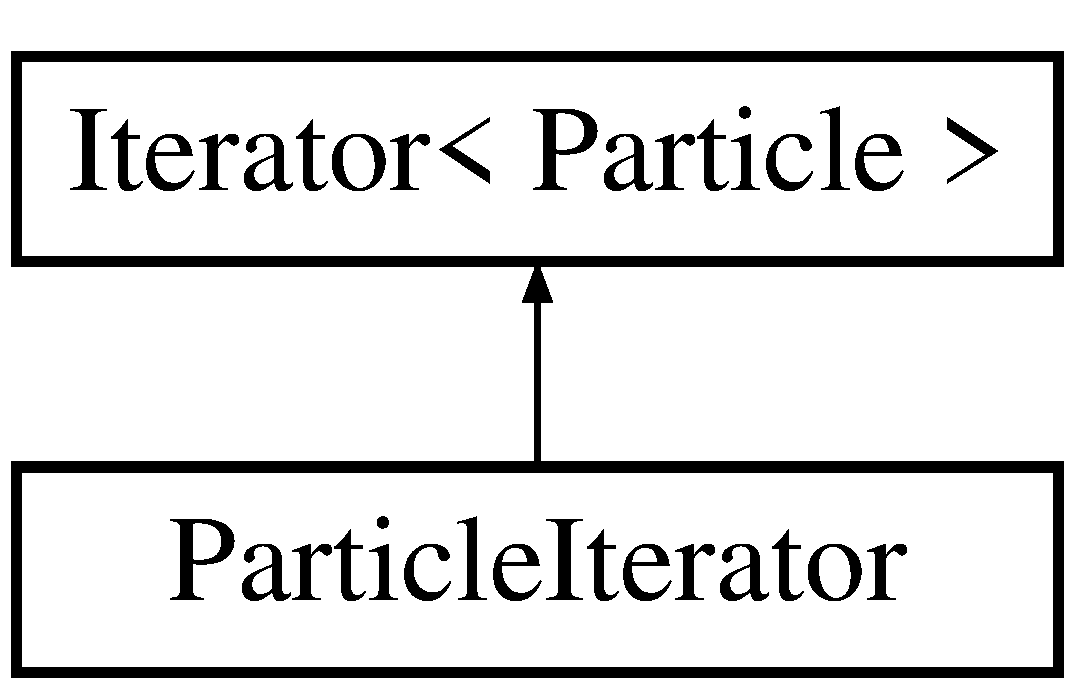
\includegraphics[height=2.000000cm]{class_particle_iterator}
\end{center}
\end{figure}
\subsection*{Additional Inherited Members}


The documentation for this class was generated from the following file\+:\begin{DoxyCompactItemize}
\item 
src/Particle.\+cpp\end{DoxyCompactItemize}

%--- End generated contents ---

% Index
\backmatter
\newpage
\phantomsection
\clearemptydoublepage
\addcontentsline{toc}{chapter}{Index}
\printindex

\end{document}
